\documentclass[conference]{IEEEtran}
\IEEEoverridecommandlockouts

\usepackage[utf8]{inputenc}
\usepackage[T1]{fontenc}
\usepackage[brazil]{babel}
\usepackage{graphicx}
\usepackage{booktabs}
\usepackage{amsmath,amssymb}
\usepackage{url}
\usepackage{listings}
\usepackage{xcolor}
\usepackage{textcomp}
\usepackage{array}

\graphicspath{{figures/}}

\definecolor{codebg}{rgb}{0.96,0.96,0.96}
\lstset{
  basicstyle=\ttfamily\scriptsize,
  backgroundcolor=\color{codebg},
  breaklines=true,
  frame=single,
  columns=fullflexible,
  keepspaces=true,
}

\begin{document}

\title{GraphQL versus REST: Um Experimento Controlado\\
sobre Tempo de Resposta e Tamanho de Payload}

\author{
\IEEEauthorblockN{Luiz Paulo Saud}
\IEEEauthorblockA{\textit{Engenharia de Software} \\
\textit{PUC Minas}\\
Belo Horizonte, Brasil}
\and
\IEEEauthorblockN{Arthur Curi}
\IEEEauthorblockA{\textit{Engenharia de Software} \\
\textit{PUC Minas}\\
Belo Horizonte, Brasil}
\and
\IEEEauthorblockN{Helio Teixeira}
\IEEEauthorblockA{\textit{Engenharia de Software} \\
\textit{PUC Minas}\\
Belo Horizonte, Brasil}
}

\maketitle

\begin{abstract}
GraphQL surge como alternativa às APIs REST, prometendo consultas mais
flexíveis e eficientes ao permitir que o cliente especifique exatamente os
dados desejados. Entretanto, os benefícios reais dessa adoção ainda carecem de
evidência empírica controlada. Este trabalho apresenta um experimento
controlado que compara as duas abordagens quanto a duas variáveis dependentes:
tempo de resposta e tamanho do payload. Ambos os paradigmas foram expostos
sobre a mesma base de dados e a mesma infraestrutura, isolando o estilo de API
como única variável independente. Foram executadas 200 medições para cada
combinação de quatro cenários de consulta e dois tratamentos, totalizando 1.600
observações. Os resultados, validados por testes não paramétricos de
Mann--Whitney com tamanho de efeito de Cliff, mostram um cenário matizado:
GraphQL reduz o tempo de resposta em até 68\% e o tamanho do payload em até 84\%
em consultas aninhadas e com seleção de campos, mas impõe sobrecarga de
processamento em consultas simples, nas quais REST se mostrou mais rápido.
Conclui-se que a superioridade de GraphQL é dependente do padrão de acesso aos
dados, e não absoluta.
\end{abstract}

\begin{IEEEkeywords}
GraphQL, REST, APIs Web, experimento controlado, desempenho, engenharia de
software experimental.
\end{IEEEkeywords}

\section{Introdução}
A linguagem de consulta GraphQL, proposta pelo Facebook como metodologia de
implementação de APIs Web, representa uma alternativa às populares APIs REST.
Baseada em grafos, a linguagem permite que clientes consultem a base de dados a
partir de \textit{schemas} tipados, especificando, num formato definido pelo
fornecedor da API, exatamente quais campos desejam receber. Em contraste, APIs
REST baseiam-se em \textit{endpoints}: operações pré-definidas, orientadas a
recursos, que retornam representações fixas dos objetos.

Desde o seu surgimento, diversos sistemas migraram de REST para GraphQL,
mantendo compatibilidade, mas buscando os benefícios da nova linguagem.
Entretanto, \textbf{não está claro quais os reais benefícios da adoção de uma
API GraphQL em detrimento de uma API REST}. Duas limitações recorrentes das
APIs REST motivam essa discussão: o \textit{over-fetching} (o servidor devolve
mais campos do que o cliente precisa) e o problema \textit{N+1} (a obtenção de
recursos relacionados exige múltiplas requisições). GraphQL promete mitigar
ambos.

O objetivo deste trabalho é realizar um experimento controlado para avaliar
quantitativamente esses benefícios, respondendo a duas questões de pesquisa:

\begin{itemize}
  \item \textbf{RQ1.} Respostas às consultas GraphQL são mais rápidas que
  respostas às consultas REST?
  \item \textbf{RQ2.} Respostas às consultas GraphQL têm tamanho menor que
  respostas às consultas REST?
\end{itemize}

\section{Desenho do Experimento}
Esta seção formaliza o desenho experimental seguindo os princípios da
engenharia de software experimental.

\subsection{Hipóteses}
Para cada questão de pesquisa formulam-se hipóteses nula ($H_0$) e alternativa
($H_1$), avaliadas por cenário de consulta:
\begin{itemize}
  \item \textbf{RQ1 -- Tempo de resposta:}
  \begin{itemize}
    \item $H1_0$: não há diferença no tempo de resposta entre GraphQL e REST
    ($\mu_{tempo}^{GraphQL} = \mu_{tempo}^{REST}$).
    \item $H1_1$: há diferença no tempo de resposta entre GraphQL e REST
    ($\mu_{tempo}^{GraphQL} \neq \mu_{tempo}^{REST}$).
  \end{itemize}
  \item \textbf{RQ2 -- Tamanho da resposta:}
  \begin{itemize}
    \item $H2_0$: não há diferença no tamanho do payload entre GraphQL e REST
    ($\mu_{tam}^{GraphQL} = \mu_{tam}^{REST}$).
    \item $H2_1$: há diferença no tamanho do payload entre GraphQL e REST
    ($\mu_{tam}^{GraphQL} \neq \mu_{tam}^{REST}$).
  \end{itemize}
\end{itemize}
Adota-se nível de significância $\alpha = 0{,}05$.

\subsection{Variáveis Dependentes}
\begin{itemize}
  \item \textbf{Tempo de resposta} (\texttt{latency\_ms}): tempo de ponta a
  ponta, em milissegundos, desde o envio da(s) requisição(ões) até o
  recebimento completo da(s) resposta(s). Para REST, em cenários aninhados,
  contabiliza-se o tempo somado de todas as requisições necessárias.
  \item \textbf{Tamanho da resposta} (\texttt{size\_bytes}): número total de
  bytes do(s) corpo(s) de resposta recebido(s).
\end{itemize}

\subsection{Variáveis Independentes}
A variável independente principal é o \textbf{estilo de API}, com dois níveis:
\textit{REST} e \textit{GraphQL}. Um segundo fator de bloqueio é o
\textbf{cenário de consulta}, com quatro níveis (descritos na
Seção~\ref{sec:cenarios}), introduzido para verificar se o efeito do estilo de
API depende do padrão de acesso aos dados.

\subsection{Tratamentos}
Os tratamentos resultam do cruzamento dos níveis: para cada cenário, executa-se
a mesma operação lógica via REST e via GraphQL. Como ambos compartilham base de
dados, processo e \textit{stack}, a única diferença sistemática entre os
tratamentos é o paradigma de API.

\subsection{Objetos Experimentais}
\label{sec:cenarios}
O objeto experimental é uma base relacional sintética e determinística
(semente fixa) com 50 usuários, 250 \textit{posts} (5 por usuário) e 2.000
comentários (8 por \textit{post}), modelando o relacionamento
\textit{usuário $\rightarrow$ post $\rightarrow$ comentário}. Sobre ela definem-se
quatro cenários:
\begin{itemize}
  \item \textbf{C1 -- Recurso único completo:} obter um usuário com todos os
  campos. Cenário de controle, sem \textit{over-fetching} nem N+1.
  \item \textbf{C2 -- Recurso único parcial:} obter apenas 3 campos de um
  usuário. Expõe o \textit{over-fetching} do REST.
  \item \textbf{C3 -- Consulta aninhada (N+1):} obter um usuário, seus
  \textit{posts} e os comentários de cada \textit{post}. Expõe o problema N+1
  do REST (1 + 1 + 5 = 7 requisições) contra uma única requisição GraphQL.
  \item \textbf{C4 -- Coleção:} obter os 50 usuários completos. Cenário de
  controle para grandes volumes sem aninhamento.
\end{itemize}

\subsection{Tipo de Projeto Experimental}
Trata-se de um projeto \textit{fatorial} $2 \times 4$ (estilo de API $\times$
cenário) com medições repetidas, executado em ambiente intra-sujeito (mesma
máquina e mesma base para todos os tratamentos).

\subsection{Quantidade de Medições}
Cada combinação (cenário $\times$ estilo) foi medida 200 vezes, precedidas de
20 execuções de aquecimento (descartadas) para estabilizar \textit{cache},
conexões persistentes e \textit{JIT}. O total é
$4 \times 2 \times 200 = 1.600$ observações, com requisições intercaladas entre
os estilos para diluir efeitos temporais.

\subsection{Ameaças à Validade}
\textbf{Validade interna:} ruído do sistema operacional e variação de
agendamento podem afetar as medições; mitigado por aquecimento, medições
repetidas, intercalação dos tratamentos e uso de estatística robusta.
\textbf{Validade de construção:} o tamanho do payload é medido em bytes do
corpo da resposta, ignorando \textit{headers} e compressão; o tempo inclui o
processamento do servidor, refletindo a experiência real do cliente.
\textbf{Validade externa:} o uso de uma base sintética e de comunicação local
(\textit{localhost}) elimina a latência de rede, podendo subestimar o ganho do
GraphQL em redes reais (onde reduzir o número de viagens e o volume de bytes é
ainda mais relevante). \textbf{Validade de conclusão:} verificou-se a
normalidade (Shapiro--Wilk) e, dada a violação frequente, optou-se por testes
não paramétricos.

\section{Preparação e Execução}
A infraestrutura foi implementada em Python. Um único servidor
(\texttt{Flask}) expõe a \emph{mesma} base de dados por duas vias: rotas REST
orientadas a recursos e um \textit{endpoint} GraphQL (\texttt{Ariadne}) com
\textit{schema} tipado e resolvedores aninhados. Um cliente
(\texttt{requests}, com sessão \textit{keep-alive}) aplica os tratamentos e
registra as variáveis dependentes em arquivo CSV. A
Listagem~\ref{lst:gql} ilustra a consulta GraphQL do cenário C3.

\begin{lstlisting}[caption={Consulta GraphQL do cenário aninhado C3.},label={lst:gql}]
query($id: ID!) {
  user(id: $id) {
    id name email
    posts {
      id title likes
      comments { id name body }
    }
  }
}
\end{lstlisting}

\subsection{Ambiente de Execução}
Os \textit{trials} foram executados em: CPU Intel64 Family 6 (28
\textit{threads} lógicas), 64\,GB de RAM, Windows 10 (build 10.0.26200),
Python 3.12.2, Flask 3.0, Ariadne 0.23 e comunicação via
\textit{loopback} (\texttt{127.0.0.1}). A semente aleatória ($42$) garante a
reprodutibilidade da base de dados.

\section{Resultados}
A Tabela~\ref{tab:resumo} consolida as medianas e o resultado dos testes de
hipótese. Todos os testes de Mann--Whitney rejeitaram $H_0$
($p \ll 0{,}001$) e apresentaram tamanho de efeito de Cliff classificado como
\textit{grande}, indicando diferenças estatística e praticamente relevantes em
todos os cenários.

\begin{table*}[t]
\centering
\caption{Medianas por cenário e tratamento, redução proporcionada pelo GraphQL
e significância (Mann--Whitney). Valores positivos de redução indicam vantagem
do GraphQL.}
\label{tab:resumo}
\begin{tabular}{llrrrrl}
\toprule
\textbf{Cenário} & \textbf{Métrica} & \textbf{REST} & \textbf{GraphQL} &
\textbf{Redução (\%)} & \textbf{$p$-valor} & \textbf{Efeito} \\
\midrule
C1 -- Recurso completo & Tempo (ms)   & 2{,}39   & 4{,}31   & $-80{,}5$  & $<0{,}001$ & grande \\
C2 -- Recurso parcial  & Tempo (ms)   & 2{,}26   & 3{,}76   & $-66{,}3$  & $<0{,}001$ & grande \\
C3 -- Aninhada (N+1)   & Tempo (ms)   & 16{,}42  & 5{,}26   & $+67{,}97$ & $<0{,}001$ & grande \\
C4 -- Coleção          & Tempo (ms)   & 2{,}64   & 5{,}96   & $-126{,}0$ & $<0{,}001$ & grande \\
\midrule
C1 -- Recurso completo & Tamanho (B)  & 554      & 574      & $-3{,}6$   & $<0{,}001$ & grande \\
C2 -- Recurso parcial  & Tamanho (B)  & 554      & 87       & $+84{,}3$  & $<0{,}001$ & grande \\
C3 -- Aninhada (N+1)   & Tamanho (B)  & 18.380   & 13.238   & $+27{,}98$ & $<0{,}001$ & grande \\
C4 -- Coleção          & Tamanho (B)  & 29.943   & 30.062   & $-0{,}4$   & $<0{,}001$ & grande \\
\bottomrule
\end{tabular}
\end{table*}

\subsection{RQ1 -- Tempo de Resposta}
A Figura~\ref{fig:lat-bars} apresenta a latência média (escala logarítmica) com
intervalos de confiança de 95\%, e a Figura~\ref{fig:lat-box} mostra a
distribuição via \textit{boxplots}. O resultado é \textbf{dependente do
cenário}:
\begin{itemize}
  \item Em consultas simples (C1, C2 e C4), REST foi significativamente mais
  rápido. A análise e validação do \textit{schema} GraphQL adicionam uma
  sobrecarga fixa de processamento que, na ausência de latência de rede,
  domina o tempo total.
  \item No cenário aninhado C3, GraphQL foi \textbf{67,97\% mais rápido} que
  REST. Aqui o problema N+1 penaliza fortemente o REST, que precisa de sete
  requisições sequenciais, enquanto o GraphQL resolve tudo em uma única
  viagem.
\end{itemize}
Portanto, rejeita-se $H1_0$ em todos os cenários, mas a \emph{direção} do
efeito favorece o GraphQL apenas quando há agregação de recursos relacionados.

\begin{figure}[t]
\centering
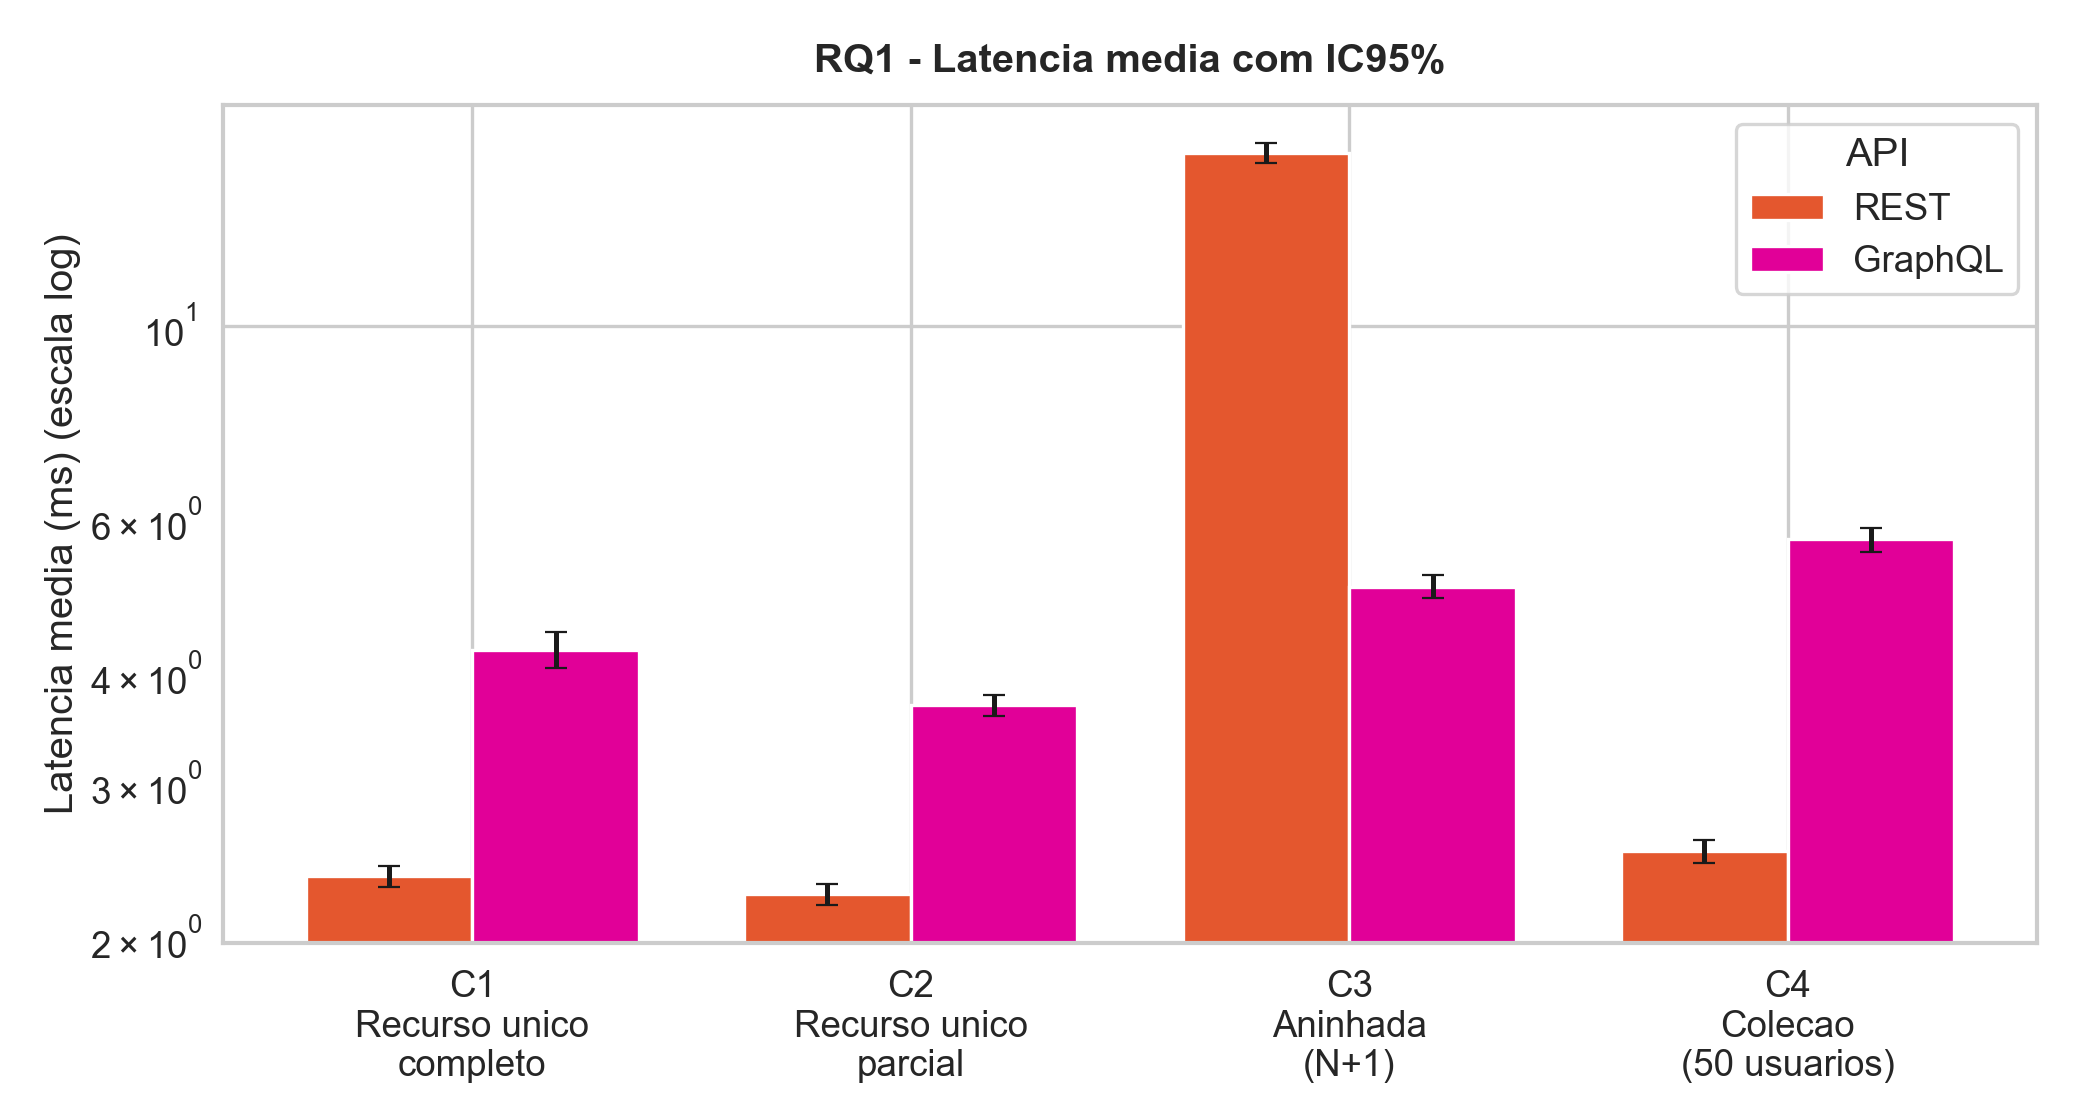
\includegraphics[width=\columnwidth]{fig_latency_bars.png}
\caption{Latência média por cenário (escala log) com IC95\%.}
\label{fig:lat-bars}
\end{figure}

\begin{figure}[t]
\centering
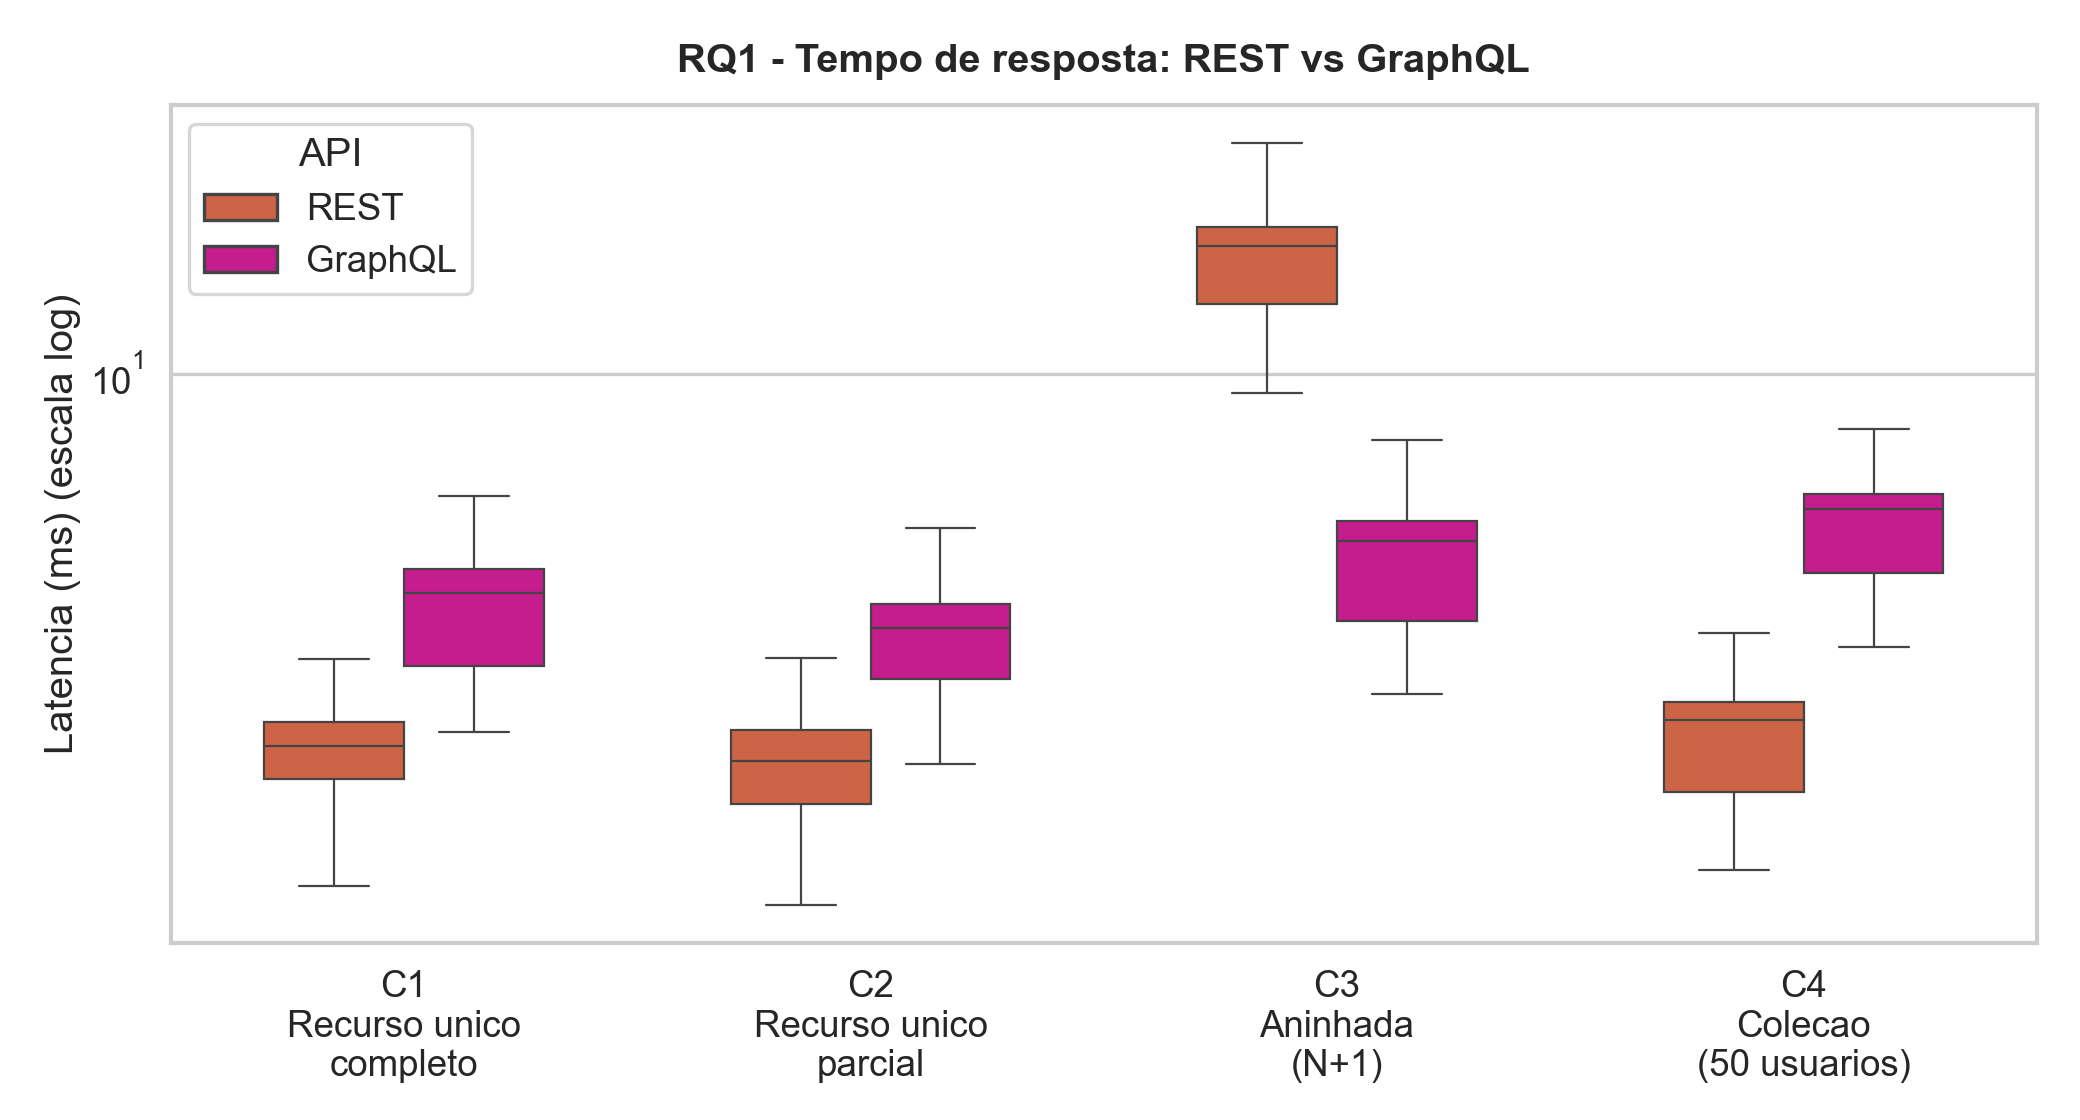
\includegraphics[width=\columnwidth]{fig_latency_box.png}
\caption{Distribuição da latência por cenário e tratamento.}
\label{fig:lat-box}
\end{figure}

\subsection{RQ2 -- Tamanho da Resposta}
As Figuras~\ref{fig:size-bars} e~\ref{fig:size-box} resumem o tamanho dos
\textit{payloads}. Novamente o efeito depende do padrão de acesso:
\begin{itemize}
  \item Em C2, a capacidade do GraphQL de selecionar campos reduziu o payload
  em \textbf{84,3\%} (de 554 para 87 bytes), eliminando o \textit{over-fetching}
  do REST.
  \item Em C3, a ausência de campos redundantes e de envelopes repetidos
  resultou em \textbf{27,98\%} menos bytes para o GraphQL.
  \item Em C1 e C4, nos quais o cliente solicita todos os campos, os tamanhos
  são praticamente equivalentes; o GraphQL chega a ser ligeiramente maior
  devido ao envelope \texttt{data} da resposta.
\end{itemize}
Rejeita-se $H2_0$ em todos os cenários, com vantagem expressiva do GraphQL
sempre que o cliente não necessita do objeto completo.

\begin{figure}[t]
\centering
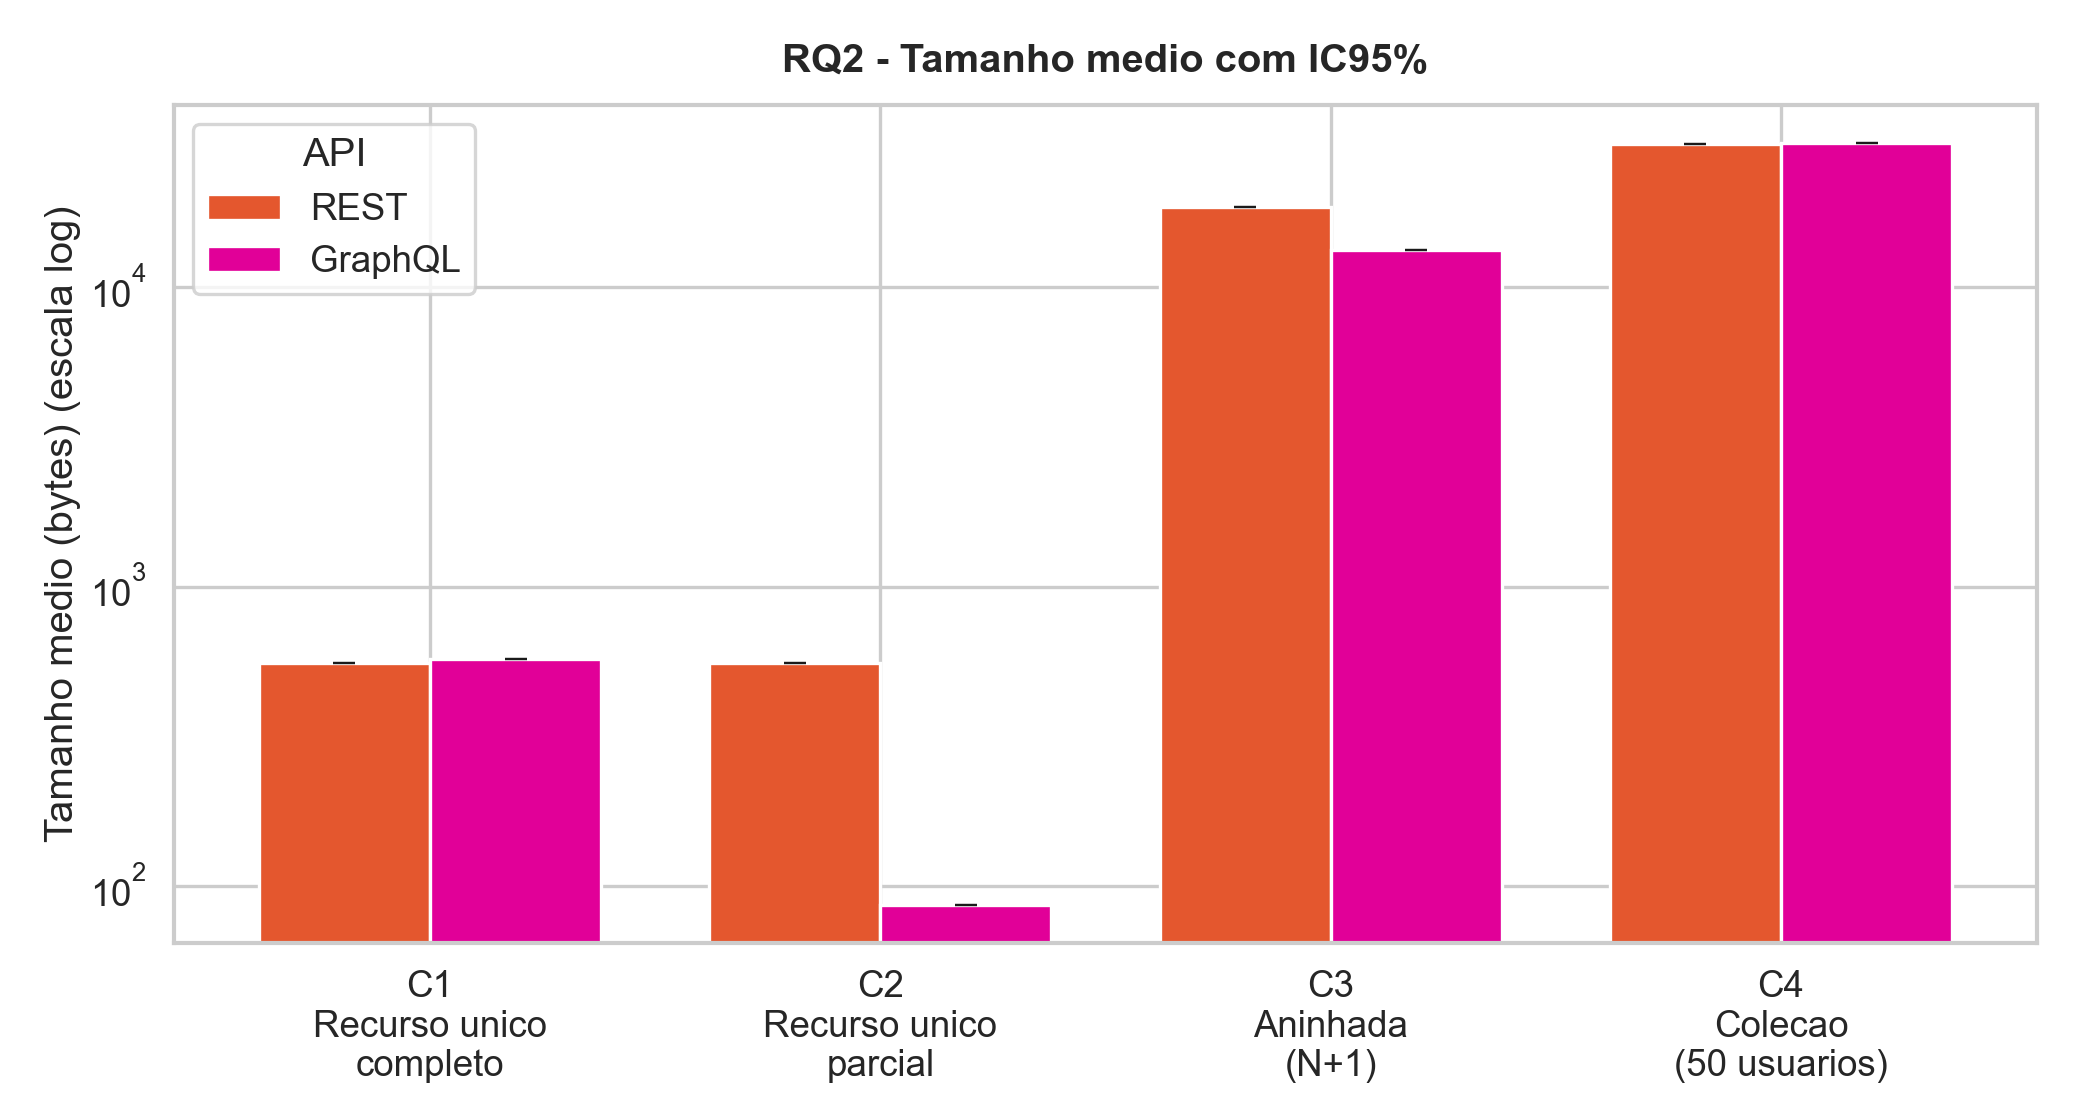
\includegraphics[width=\columnwidth]{fig_size_bars.png}
\caption{Tamanho médio do payload por cenário (escala log) com IC95\%.}
\label{fig:size-bars}
\end{figure}

\begin{figure}[t]
\centering
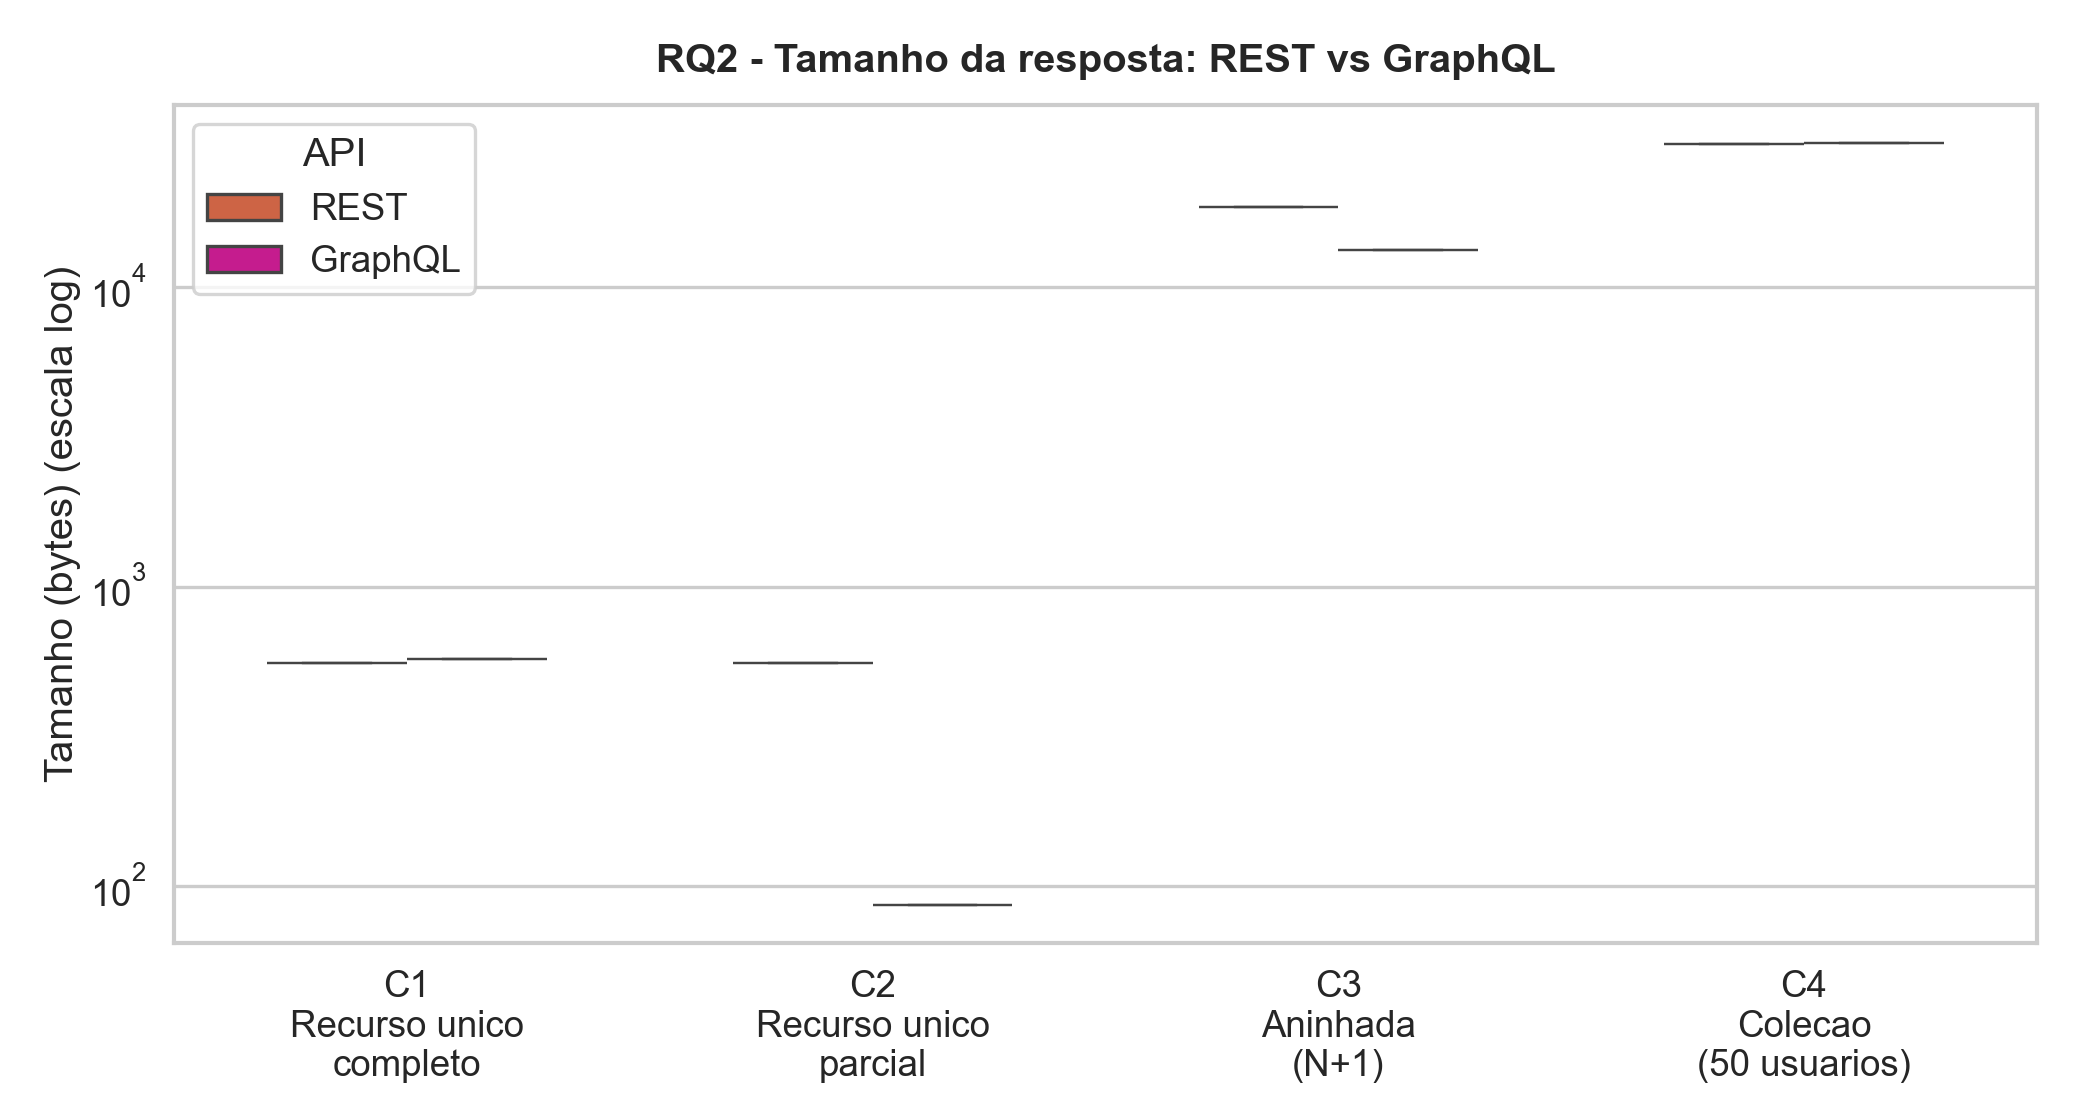
\includegraphics[width=\columnwidth]{fig_size_box.png}
\caption{Distribuição do tamanho do payload por cenário e tratamento.}
\label{fig:size-box}
\end{figure}

\section{Discussão}
Os dados desautorizam tanto a visão de que ``GraphQL é sempre superior'' quanto
a de que ``GraphQL é apenas \textit{hype}''. A vantagem do GraphQL é
\textbf{condicional ao padrão de acesso aos dados}:

\textbf{GraphQL vence claramente} quando (i) o cliente precisa de um subconjunto
dos campos (combatendo \textit{over-fetching}, RQ2/C2) ou (ii) precisa agregar
recursos relacionados em uma única operação (combatendo o N+1, RQ1/C3). Esses
são exatamente os casos que motivaram a criação da linguagem, e os ganhos
medidos (até $-84\%$ em bytes e $-68\%$ em tempo) são substanciais.

\textbf{REST vence} em consultas simples de recurso único ou coleção completa,
nas quais não há over-fetching nem aninhamento. Nesses casos, a sobrecarga de
\textit{parsing} e validação do \textit{schema} GraphQL não é compensada por
nenhuma economia de viagens ou de dados.

Vale destacar que o experimento foi conduzido em \textit{loopback}, sem latência
de rede. Em ambientes reais, o custo de cada viagem adicional (RTT) e de cada
byte trafegado é muito maior; logo, espera-se que a vantagem do GraphQL nos
cenários C2 e C3 seja \emph{ainda mais pronunciada}, enquanto a desvantagem nos
cenários simples tende a se diluir frente ao RTT de rede.

\section{Conclusão}
Este experimento controlado comparou GraphQL e REST quanto a tempo de resposta
e tamanho de payload, sob infraestrutura e base de dados idênticas, em 1.600
medições. Quanto à RQ1, GraphQL \emph{não} é universalmente mais rápido: vence
em consultas aninhadas (até 68\% menos tempo), mas perde em consultas simples
devido à sobrecarga de processamento. Quanto à RQ2, GraphQL produz respostas
menores sempre que o cliente seleciona um subconjunto dos dados (até 84\% menos
bytes), sendo equivalente quando todos os campos são solicitados. A conclusão
central é que a decisão entre GraphQL e REST deve ser guiada pelo
\textbf{padrão de consumo de dados da aplicação}: APIs com clientes
heterogêneos, telas ricas e dados altamente relacionados tendem a se beneficiar
do GraphQL, enquanto serviços simples e orientados a recursos podem permanecer
mais eficientes com REST. Como trabalhos futuros, sugere-se replicar o
experimento sobre rede real, incluir compressão (\textit{gzip}) e avaliar o
custo de servidor (CPU/memória) sob carga concorrente.

\begin{thebibliography}{00}
\bibitem{graphql} GraphQL Foundation, ``GraphQL Specification,'' 2021.
[Online]. Disponível em: \url{https://spec.graphql.org/}
\bibitem{fielding} R. T. Fielding, ``Architectural Styles and the Design of
Network-based Software Architectures,'' Tese de Doutorado, Univ. of California,
Irvine, 2000.
\bibitem{brito} G. Brito and M. T. Valente, ``REST vs GraphQL: A Controlled
Experiment,'' in \textit{IEEE Int. Conf. on Software Architecture (ICSA)}, 2020.
\bibitem{wohlin} C. Wohlin et al., \textit{Experimentation in Software
Engineering}. Springer, 2012.
\end{thebibliography}

\end{document}
